\section{Synthèse FRF}

% Implementation
\begin{frame}{Synthèse dans le domaine fréquentiel}

 \begin{itemize}
  \item Admittance au chevalet
  \( \frac{1}{Y_{total}} = \frac{1}{Y_{body}} + \frac{1}{Y_{string}} \),
  
  \item Fonction de transfert du système
  \( \frac{\delta_{bridge}}{F_{excitation}} = \frac{Y_{total}H}{j\omega} \),

  \item Excitation :
  	\begin{itemize}
	 \item Par une impulsion,
	 \item Ou par créneau : force excitatrice longue.
     \end{itemize}

   
 \end{itemize}
\end{frame}

% Résultats
\begin{frame}{Résultats}

	\begin{itemize}
		\item 6 cordes synthétisables,
		\item Besoin d'un nombre de modes élevé pour le modèle de la corde,
		\item Proportion entre corde et corps.
		
	\end{itemize}
	 \begin{figure}
		\centering
		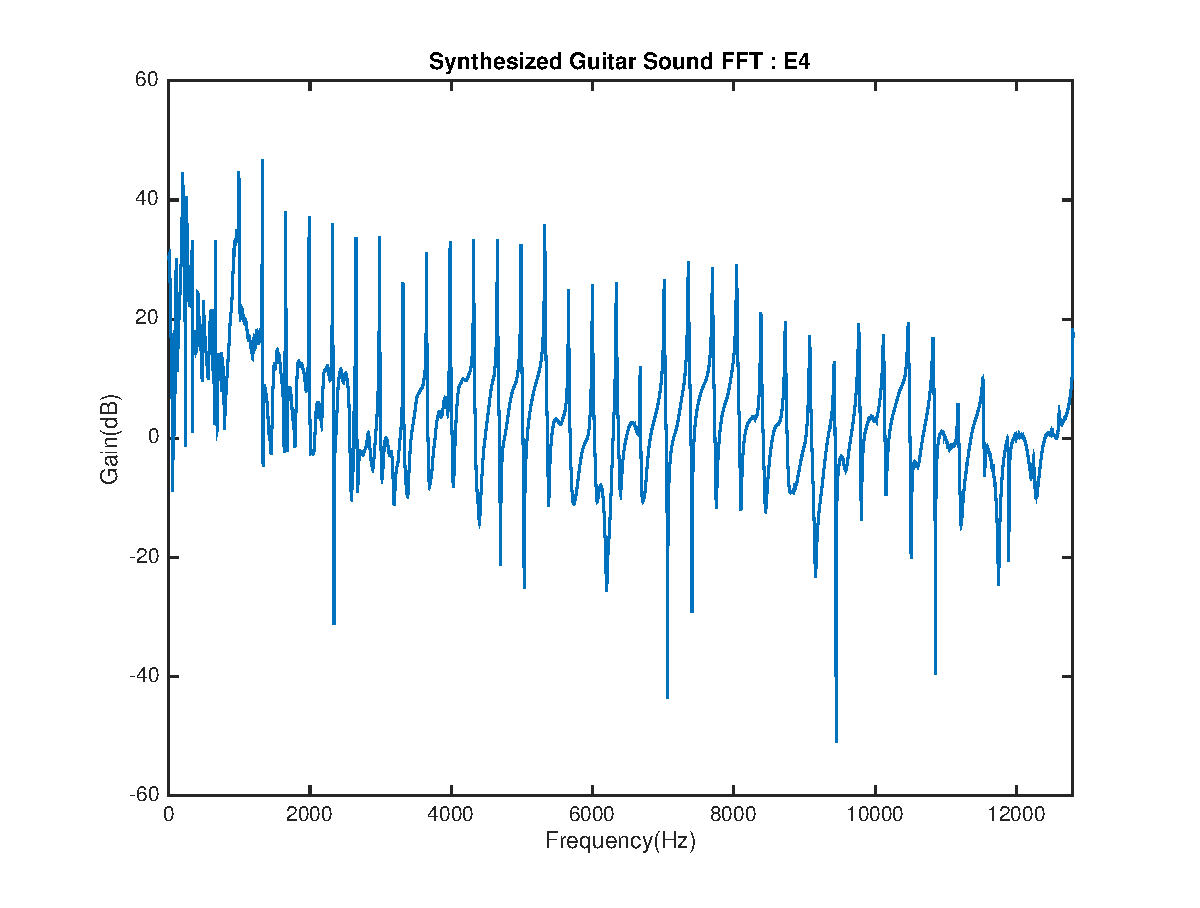
\includegraphics[width=8cm,height=4cm]{figures/frf_synthesized_sound_E4.eps}
	\end{figure}
\end{frame}